%!TEX root = ../main.tex

\chapter{Project plan}
\label{cha:plan}

\section{Improving the debugging experience}

The plan for improving Gillian's debugger more or less follows on from the
evaluation of the previous one~\cite{gillian-debugging-2021}. Here are some
primary objectives for this project; of course, these are subject to change as
work continues:

\begin{itemize}

  \item As stated in \autoref{sec:intro}, the DAP doesn't have the command set
        necessary for debugging symbolic execution. We can, however, use a
        combination of Webviews and custom DAP requests / events to supplement
        the existing debugging UI, as outlined in \autoref{sec:vscode}; this
        will be a necessity to develop many of the other features on this list.

  \item A prime missing feature as the debugger stands is the ability for users
        to select branches of execution when debugging. Currently, the debugger
        runs through the problem top-to-bottom, dealing with each branch in
        turn. Ideally, users will able to select which branch to go down when
        given a choice. As a bare minimum, this should be implemented for
        if-else statements; ideally, this should be extended to cover switch
        statements, as well as any other branching statements in the target
        languages supported.

\begin{figure}
  \noindent
  \makebox[\textwidth]{
    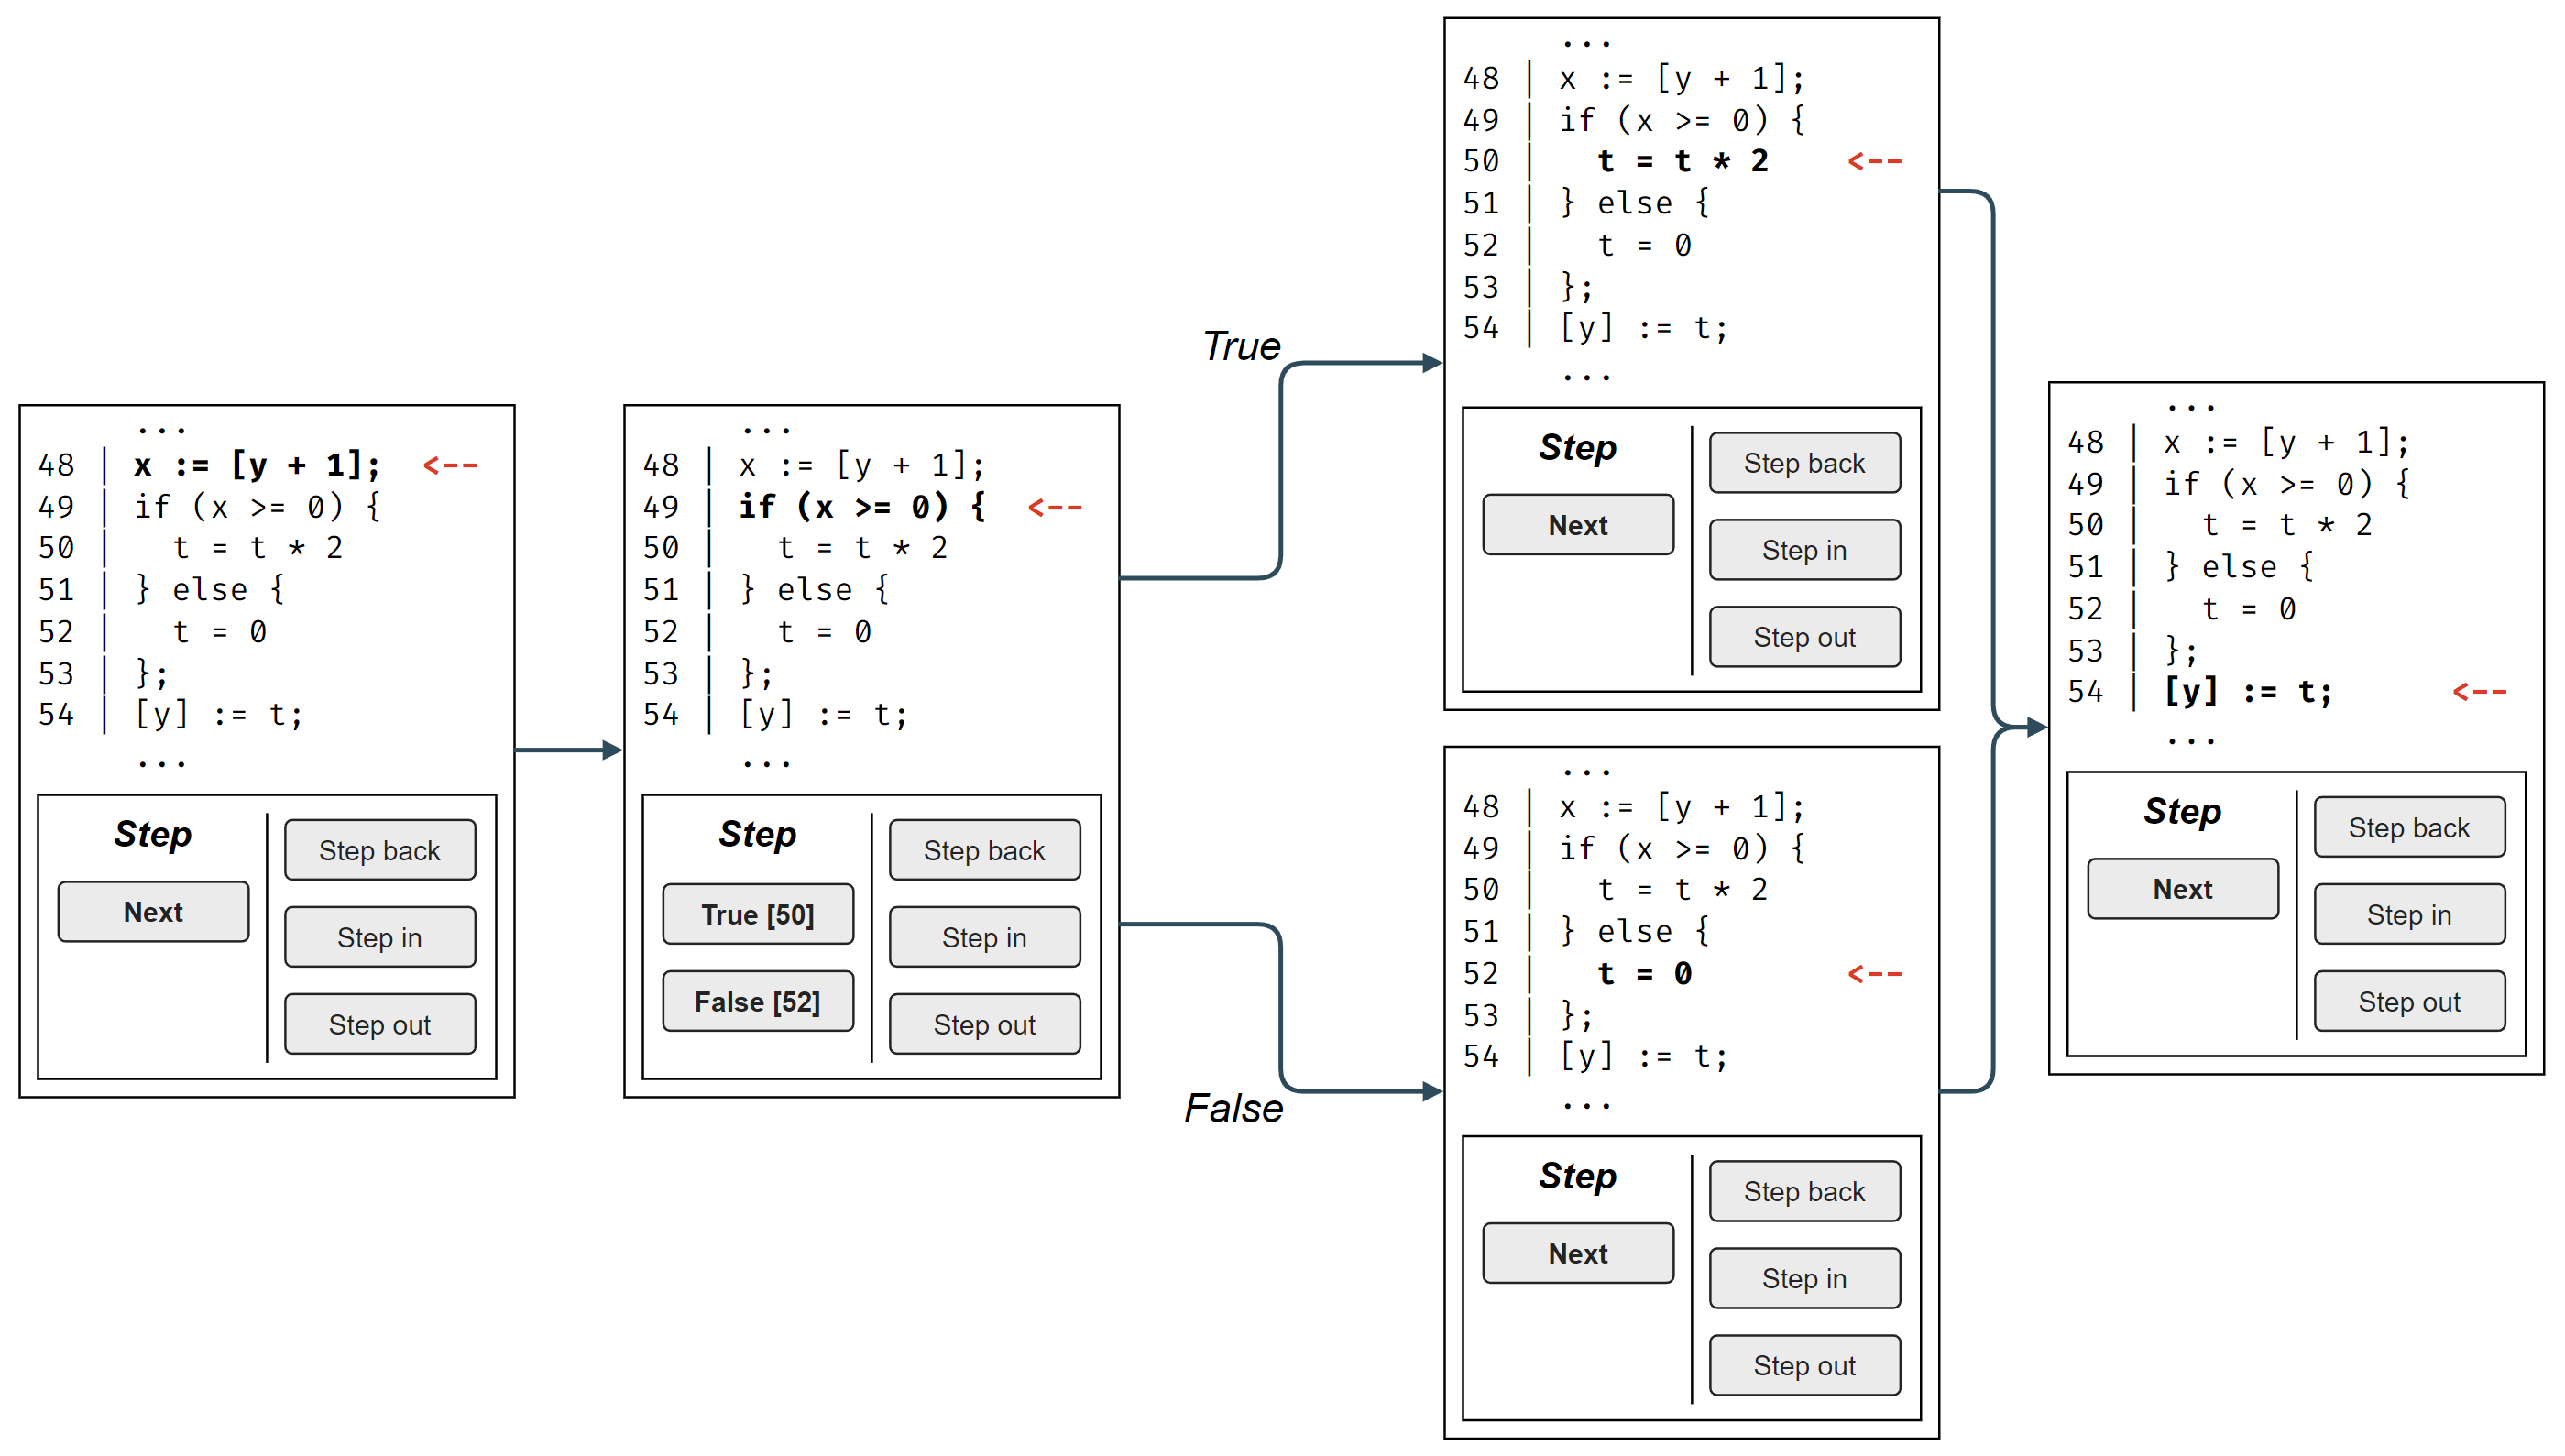
\includegraphics[width=500px]{img/branch-selection-mockup.png}
  }
  \caption{A mock-up of a potential UI flow for selecting execution branch.}
  \label{fig:branch-selection-mockup}
\end{figure}

% Maybe run an HTTP server when debugging to serve the extra info and controls?

  % Thanks sacha!
  \item A desired feature is the ability to step through Gillian's unification
        process, which stands as one of the pain points of the current user
        experience; a large share of verification errors occur when unifying
        against either the pre-condition of a called function, or the
        post-condition of the current function. In the presence of several
        specifications, the process of identifying which specs \textit{should}
        be unifying (but aren't) often takes a significant amount of time and
        thought, when a bespoke interface would greatly streamline this process.

        In particular, unification is performed following tree-shaped
        \textit{unification plans}; the ability to step through and visualise
        progress in these plans would immediately give the developer a far
        better idea of a unification error's cause.

  \item As stated in the evaluation of the previous project, the debugger is
        entirely focused on symbolic execution errors. To turn Gillian's
        debugger into a tool that can be comfortably used by real developers,
        having the debugger encompass more error types should be worked towards.

  \item A natural extension of being able to select branches of execution is a
        full tree visualisation of execution paths, allowing developers to jump
        forwards or backwards (or 'sideways', in a sense) to any step of
        execution.

  \item Potentially, small details such as showing resources that have been
        freed, à la VeriFast, could be implemented; this purely depends on
        available time, and what would and wouldn't be deemed useful by
        Gillian's primary developers and users.

  \item A potential goal for this project is implementing Gillian debugging for
        the Rust programming language~\cite{rust}. This is not a certainty, as
        it depends both on how much time is available, and on the progress of
        another final year project taking place in parallel with this one.

\end{itemize}

\section{Rough project timeline}

\newcommand{\vertline}{\color{black}\makebox[0pt]{\textbullet}\hskip-0.5pt\vrule width 1pt\hspace{\labelsep}}

\begin{flushleft}
\begin{tabular}{@{\,}r <{\hskip 2pt} !{\vertline} >{\raggedright\arraybackslash}p{13cm}}

  March & Implement stepping through unification plans         \newline \\
  April & Implement custom debugging UI for VSCode             \newline
          Including branching execution and tree visualisation \newline \\
  May   & Implement quality-of-life changes                    \newline
          Implement Rust debugging (if possible)               \newline \\
  June  & Finish implementation, finalize report               \newline \\
  
\end{tabular}
\end{flushleft}
